\section{Problem Statement and Motivation}

Consider a conductive element with length $L$, cross-sectional area $A$, and resistivity $\rho$. 
Its electrical resistance is given by

\begin{equation}
    R = \frac{\rho L}{A}.
\end{equation}

Under mechanical loading, both the geometry and the intrinsic material properties of the conductor may change. 
In particular, the length, cross-sectional area, and resistivity become functions of deformation, 
making the resistance dependent on the mechanical state.

Using Ohm's law,

\begin{equation}
    R = \frac{V}{I},
\end{equation}

and expressing voltage and current in terms of field quantities,

\begin{equation}
    V = EL, \qquad I = JA,
\end{equation}

we obtain

\begin{equation}
    \frac{EL}{JA} = \frac{\rho L}{A}.
\end{equation}

Canceling the geometric factors $L$ and $A$ leads to the local relation

\begin{equation}
    \mathbf{J} = \sigma \mathbf{E}, \qquad \sigma = \frac{1}{\rho},
\end{equation}

where $\mathbf{E} = -\nabla V$ is the electric field. 
This formulation expresses Ohm’s law in a local (continuum) form, independent of the specific geometry 
and applicable to spatially varying fields.

Combining this with charge conservation in the steady state,

\begin{equation}
    \nabla \cdot \mathbf{J} = 0,
\end{equation}

yields the conductivity equation

\begin{equation}
    \nabla \cdot (\sigma \nabla V) = 0.
\end{equation}

This equation provides a continuum description of electrical conduction in materials, 
where the conductivity $\sigma$ may vary spatially. It belongs to the class of elliptic partial differential equations 
in divergence form \cite{evans}.

In piezoresistive materials, the key feature is that the conductivity is no longer constant, but depends on the mechanical deformation of the material. 
At a macroscopic level, this dependence can be expressed as

\begin{equation}
    \sigma = \sigma(\varepsilon(u)),
\end{equation}

where the strain tensor is given by\footnote{The strain tensor is defined as the symmetric part of the displacement gradient, which removes rigid body rotations and captures the true deformation of the material.}

\begin{equation}
    \varepsilon(u) = \frac{1}{2}(\nabla u + \nabla u^T).
\end{equation}

This relation can be interpreted as an effective description of how mechanical deformation influences electrical transport. 
From a physical perspective, the dependence of conductivity on strain originates from strain-induced modifications of the electronic structure 
and carrier transport properties, which are affected by lattice deformation \cite{hamaguchi}.

The resulting model therefore introduces a nonlinear coupling between mechanical deformation and electrical conduction: 
the mechanical field $u$ determines the strain $\varepsilon(u)$, which modifies the conductivity $\sigma$, and this in turn affects 
the electrical potential $V$ through the conductivity equation.

\begin{figure}[htbp]
    \centering
    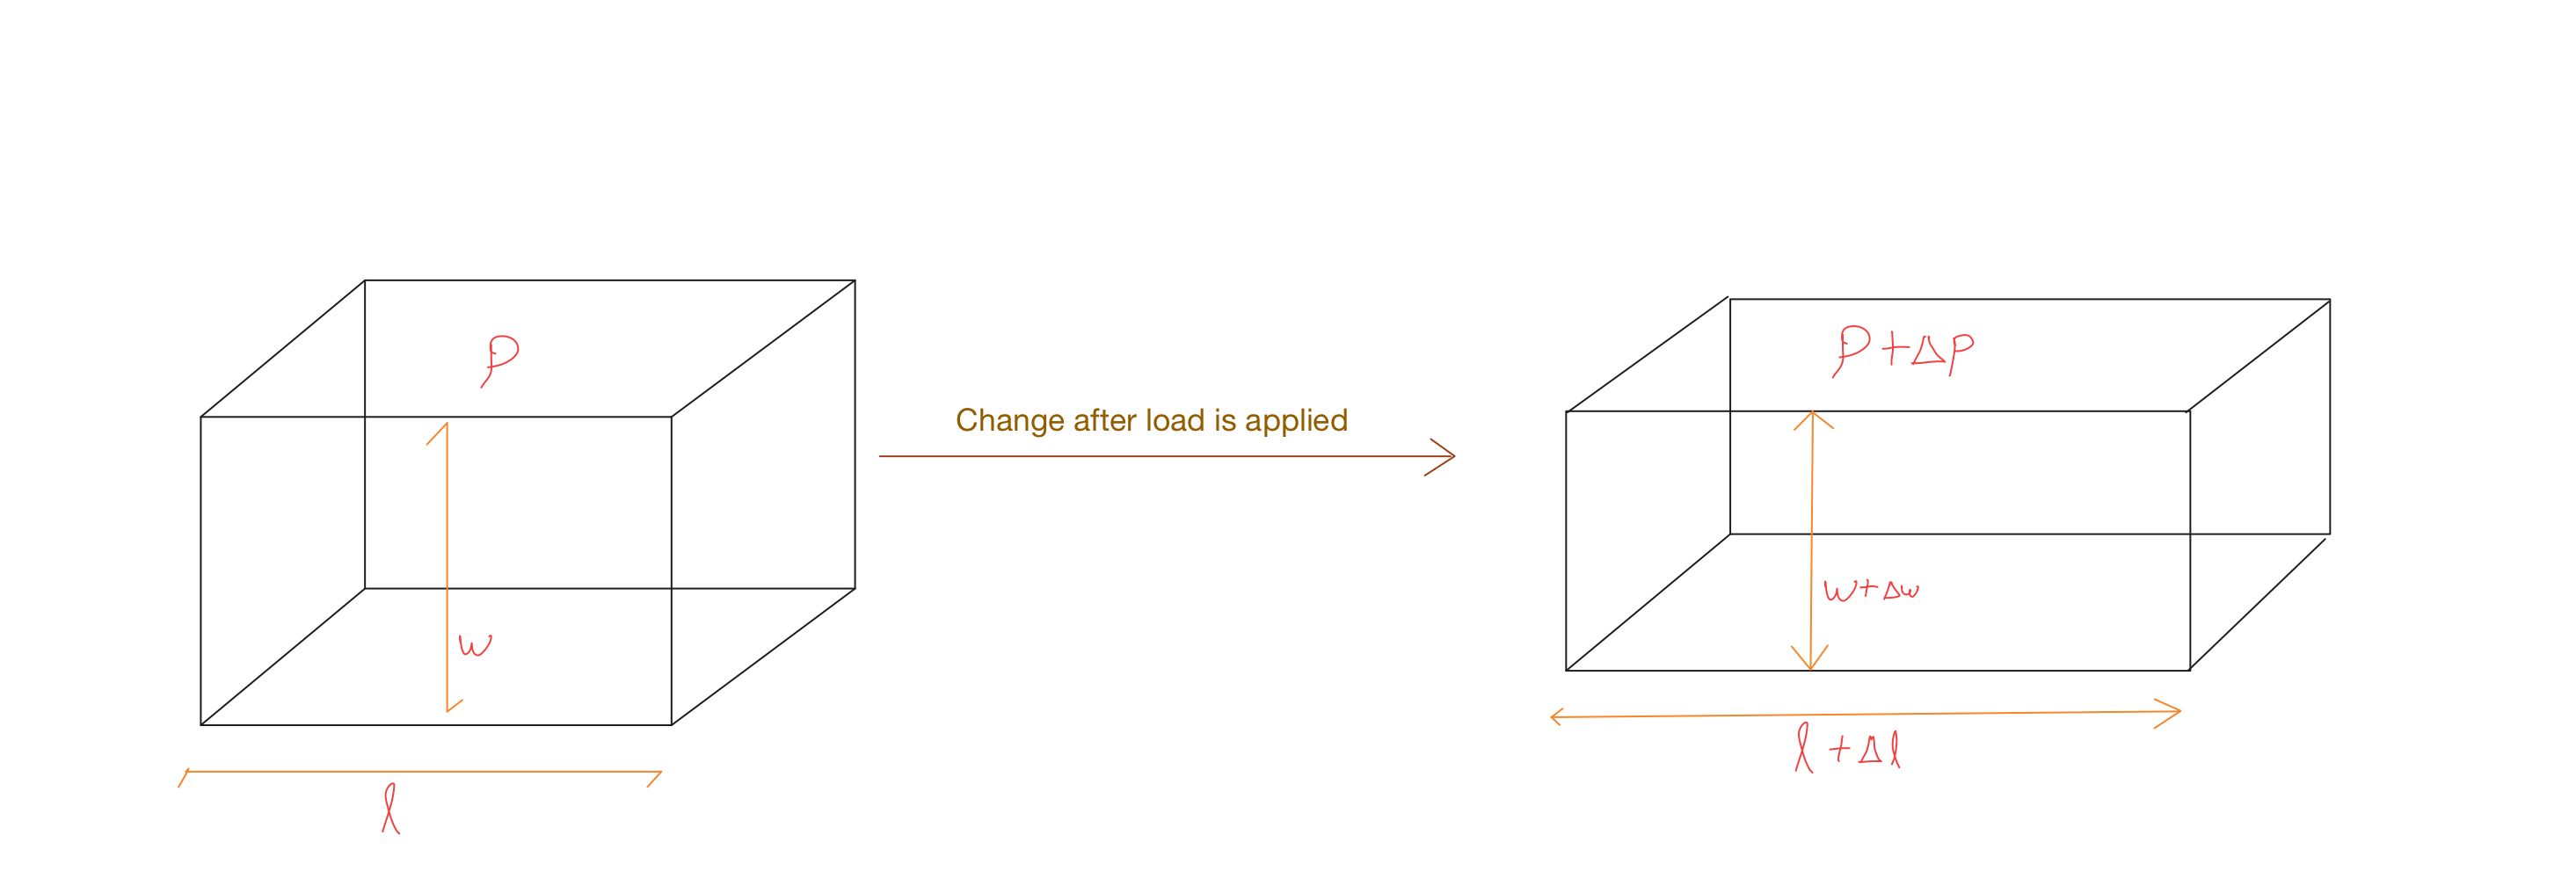
\includegraphics[width=0.7\textwidth]{Images/model1.png}
    \caption{Change of geometric and material properties under mechanical deformation. 
    $L$ denotes the length of the conductor, $W$ its characteristic width, and $A = W^2$ the cross-sectional area (assuming a square cross-section). 
    The material property $\rho$ represents the electrical resistivity, which may vary under mechanical deformation. 
    Both geometric changes and intrinsic material variations contribute to the overall change in resistance.}
\end{figure}

This illustrates that both geometric deformation and intrinsic material changes contribute to the variation of resistance, 
providing the basis for modeling the piezoresistive effect within a continuum framework.